Coloca los siguientes elementos en el lugar que le correspondan a la imagen de la Vía Láctea.

\begin{center}
    \dashedbox{Halo gal\'actico} \quad \dashedbox{10,000 a\~nos luz} \quad \dashedbox{Núcleo gal\'actico} \quad \dashedbox{100,000 a\~nos luz}
\end{center}
\begin{figure}[H]
    \centering
    \ifprintanswers
    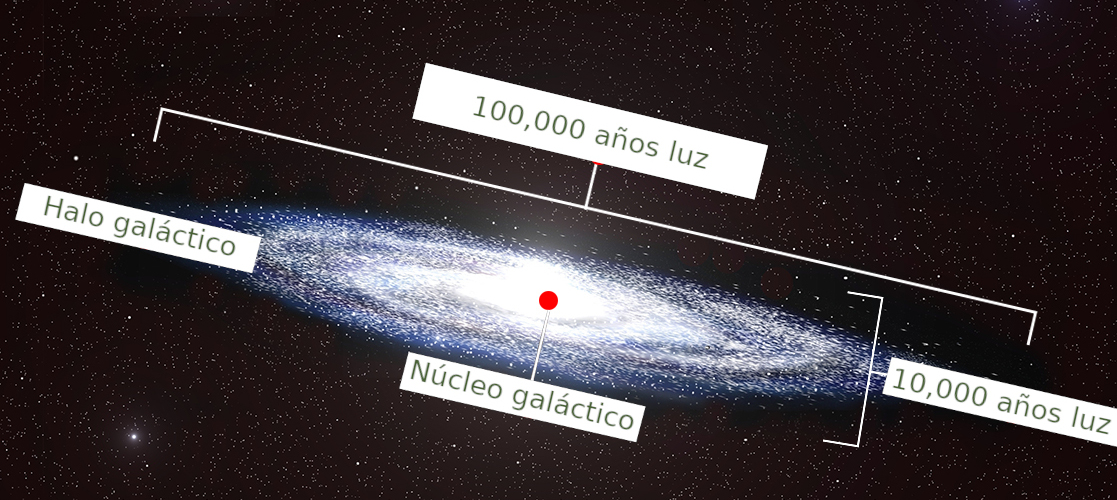
\includegraphics[width=0.75\textwidth]{../images/SINFI_AC85_IMG1_oka.jpg}
    \else
    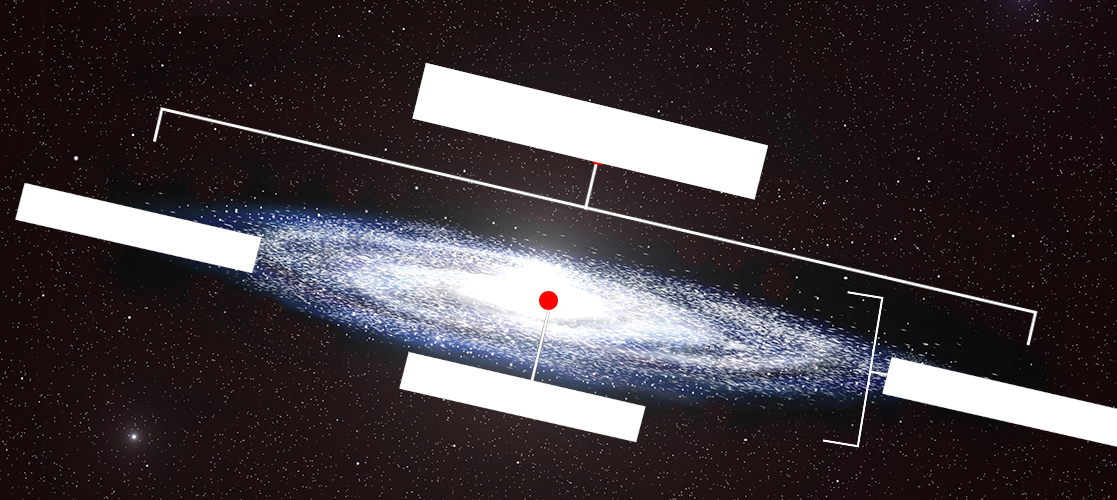
\includegraphics[width=0.75\textwidth]{../images/SINFI_AC85_IMG1_ok.jpg}
    \fi
\end{figure}

